\chapter{Daoism, Popular Religion and the Cosmos}

\section{Daoism as a philosophy}

Daoism (\zht{道家}, Dàojiā, ``the school of the Way'') offered the main alternative to
Confucian activism. Where Confucians wanted to fix society through ritual and study,
Daoists argued that such efforts are themselves the problem: they distort the natural
spontaneity of things.

\subsection{The texts}

\begin{itemize}
  \item \textbf{\emph{Daodejing}} (\zht{道德經}, ``Classic of the Way and its Power''),
        attributed to \textbf{Laozi} (\zht{老子}, ``Old Master''), traditionally an older
        contemporary of Confucius. Most scholars think the text was compiled over time,
        reaching its present form around the 4th--3rd century BCE. Eighty-one short,
        poetic chapters.
  \item \textbf{\emph{Zhuangzi}} (\zht{莊子}), named after Zhuang Zhou (4th c.\ BCE):
        witty prose full of parables, paradoxes and talking animals.
\end{itemize}

\subsection{Key concepts}

\begin{center}
\begin{tabular}{llp{8.5cm}}
\toprule
Term & Pinyin & Meaning \\
\midrule
\zht{道} & dào & the Way: the nameless source and pattern of all things; ``the Dao that can be spoken of is not the constant Dao'' \\
\zht{德} & dé & the power or virtue a thing has when it follows the Dao \\
\zht{無為} & wúwéi & ``non-action'': acting without forcing, effortless action in harmony with nature \\
\zht{自然} & zìrán & ``self-so'', spontaneity, naturalness \\
\zht{樸} & pǔ & the uncarved block: simplicity before social conditioning \\
\bottomrule
\end{tabular}
\end{center}

\begin{example}[Water as the model]
The \emph{Daodejing} repeatedly praises water: it is the softest thing, it takes the lowest
place, yet nothing can resist it and it wears away stone. The Daoist sage, like water,
yields and does not contend, and therefore is not defeated. Compare the Confucian image of
the junzi as upright and firm.
\end{example}

\begin{example}[Zhuangzi's butterfly]
Zhuangzi dreamed he was a butterfly, happily fluttering about, not knowing he was Zhuang
Zhou. He woke up and was Zhuang Zhou. He did not know whether he was Zhou who had dreamed
of being a butterfly, or a butterfly dreaming of being Zhou. The story questions fixed
identities and the boundary between perspectives.
\end{example}

\begin{example}[Cook Ding]
A cook carving an ox does not hack at bones; he lets his blade follow the natural joints,
so that after nineteen years it is as sharp as new. Mastery is a matter of following the
inherent structure of things: a picture of \emph{wuwei} in action.
\end{example}

\subsection{Confucianism and Daoism compared}

\begin{center}
\begin{tabular}{lll}
\toprule
 & Confucianism & Daoism \\
\midrule
Focus & society, family, government & nature, the individual, the cosmos \\
Ideal person & junzi (cultivated gentleman) & sage / ``true person'' (\zht{真人}) \\
Method & study, ritual, effort & non-action, simplicity, spontaneity \\
Attitude to rules & necessary, civilizing & artificial, distorting \\
Typical symbol & the teacher, the ancestral hall & water, the uncarved block, the valley \\
Political role & ideology of officials & refuge of officials out of office \\
\bottomrule
\end{tabular}
\end{center}

\begin{important}[``Confucian in office, Daoist in retirement'']
The two were not usually rival identities. A scholar-official could serve the state as a
Confucian and write Daoist-flavoured nature poetry in retirement (Tao Yuanming, Li Bai).
Most Chinese drew on both, plus Buddhism: ``the three teachings are one''
(\zht{三教合一}).
\end{important}

\section{Yin--yang and the five phases}

Underlying both schools is a shared correlative cosmology developed in the Warring States
and Han.

\subsection{Yin and yang}

\emph{Yin} (\zht{陰}) and \emph{yang} (\zht{陽}) are complementary, interdependent forces,
not good and evil. Originally the shady and sunny sides of a hill.

\begin{center}
\begin{tabular}{ll}
\toprule
Yin \zht{陰} & Yang \zht{陽} \\
\midrule
dark, shade & light, sun \\
female & male \\
earth & heaven \\
passive, receptive & active, creative \\
moon, water, cold & sun, fire, heat \\
even numbers & odd numbers \\
\bottomrule
\end{tabular}
\end{center}

\subsection{The five phases}

The \emph{five phases} are \zht{五行} (wǔxíng).

Wood, fire, earth, metal and water are not ``elements'' (substances) but \emph{phases} of
change, linked in generating and overcoming cycles. They were correlated with seasons,
directions, colours, organs, dynasties and much more.

\begin{center}
\begin{tikzpicture}[ph/.style={circle, draw, thick, minimum size=1.5cm, align=center, font=\small}]
  \node[ph, fill=green!20] (wood) at (90+72*0:2.6) {Wood\\\zht{木}};
  \node[ph, fill=red!20] (fire) at (90-72*1:2.6) {Fire\\\zht{火}};
  \node[ph, fill=yellow!35] (earth) at (90-72*2:2.6) {Earth\\\zht{土}};
  \node[ph, fill=gray!20] (metal) at (90-72*3:2.6) {Metal\\\zht{金}};
  \node[ph, fill=blue!20] (water) at (90-72*4:2.6) {Water\\\zht{水}};
  % generating cycle (outer)
  \draw[->, thick, green!50!black] (wood) to[bend left=20] (fire);
  \draw[->, thick, green!50!black] (fire) to[bend left=20] (earth);
  \draw[->, thick, green!50!black] (earth) to[bend left=20] (metal);
  \draw[->, thick, green!50!black] (metal) to[bend left=20] (water);
  \draw[->, thick, green!50!black] (water) to[bend left=20] (wood);
  % overcoming cycle (star)
  \draw[->, thick, red!70!black, dashed] (wood) -- (earth);
  \draw[->, thick, red!70!black, dashed] (earth) -- (water);
  \draw[->, thick, red!70!black, dashed] (water) -- (fire);
  \draw[->, thick, red!70!black, dashed] (fire) -- (metal);
  \draw[->, thick, red!70!black, dashed] (metal) -- (wood);
  \node[font=\scriptsize, green!50!black, anchor=west] at (3.6,1.2) {solid: generates};
  \node[font=\scriptsize, red!70!black, anchor=west] at (3.6,0.7) {dashed: overcomes};
\end{tikzpicture}
\end{center}

\begin{itemize}
  \item Generating: wood feeds fire; fire makes ash (earth); earth bears metal; metal
        collects dew (water); water nourishes wood.
  \item Overcoming: wood (roots) breaks earth; earth dams water; water quenches fire; fire
        melts metal; metal (axe) cuts wood.
  \item Dynasties claimed a phase: the Qin claimed water (colour black) to overcome the
        Zhou's fire.
\end{itemize}

\begin{aside}
This cosmology spread across East Asia: the Korean flag (\ko{태극기}, Taegukgi) shows a
red--blue yin--yang circle surrounded by four trigrams from the \emph{Book of Changes}
(\zht{易經}, Yìjīng). Japanese \emph{onmyōdō} (\ja{陰陽道}, ``way of yin and yang'') was a
court bureau of diviners in the Heian period, a topic that reappears in EASIA 120R's
lectures on Abe no Seimei.
\end{aside}

\section{Religious Daoism}

From the late Han, Daoism also became an organized religion (\zht{道教}, Dàojiào), with
priests, scriptures, temples and a vast pantheon. Students often confuse this with the
philosophy; the two overlapped but are distinct.

\begin{itemize}
  \item \textbf{Way of the Celestial Masters} (2nd c.\ CE): founded by Zhang Daoling, who
        claimed revelation from a deified Laozi. A church-like community with priests,
        confession of sins and healing.
  \item \textbf{Immortality}: the search for physical immortality through breathing
        exercises, diet, meditation and alchemy (several emperors died from elixirs
        containing mercury). The immortals (\zht{仙}, xiān) became popular figures.
  \item \textbf{Canon}: the Daoist Canon (\zht{道藏}) grew to over 1400 texts by the Ming.
  \item \textbf{Quanzhen} (``Complete Perfection'', 12th c.): monastic Daoism influenced by
        Chan Buddhism.
\end{itemize}

\section{Popular religion}

Most people in premodern China did not identify with a single religion. ``Chinese popular
religion'' mixed elements from all three teachings with local cults.

\begin{center}
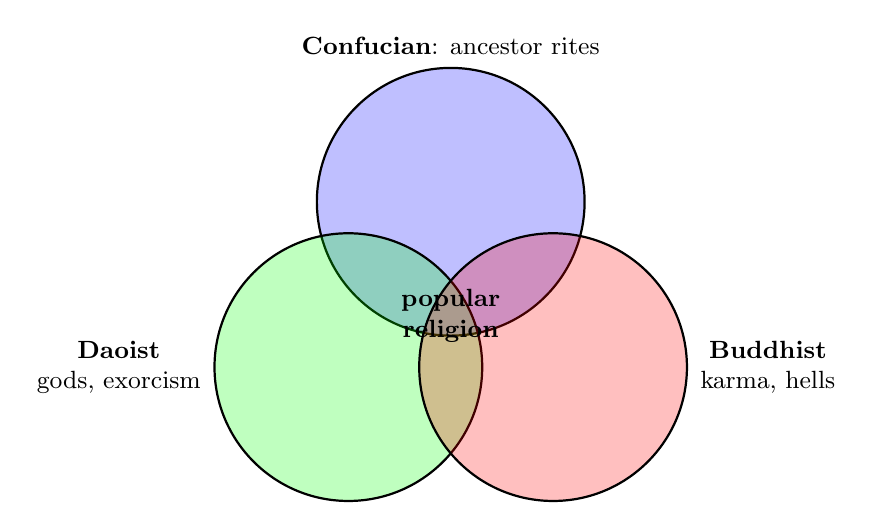
\begin{tikzpicture}[c/.style={circle, draw, thick, minimum size=3.4cm, align=center, font=\small, fill opacity=0.25, text opacity=1}]
  \node[c, fill=blue] (co) at (0,1.2) {};
  \node[c, fill=green] (da) at (-1.3,-0.9) {};
  \node[c, fill=red] (bu) at (1.3,-0.9) {};
  \node[font=\small, align=center, anchor=south] at (0,2.95) {\textbf{Confucian}: ancestor rites};
  \node[font=\small, align=center, anchor=east] at (-3.05,-0.9) {\textbf{Daoist}\\gods, exorcism};
  \node[font=\small, align=center, anchor=west] at (3.05,-0.9) {\textbf{Buddhist}\\karma, hells};
  \node[font=\small\bfseries, align=center] at (0,-0.25) {popular\\religion};
\end{tikzpicture}
\end{center}

\begin{itemize}
  \item \textbf{Ancestor veneration}: household altars, tablets, offerings on death
        anniversaries and at Qingming (``tomb-sweeping'').
  \item \textbf{Gods as bureaucrats}: the Jade Emperor rules a celestial bureaucracy that
        mirrors the earthly one; the Kitchen God reports on the family each New Year (so
        families smeared his lips with sweets).
  \item \textbf{Ghosts}: the dead without descendants become ``hungry ghosts'' who must be
        fed during the Ghost Festival (7th lunar month).
  \item \textbf{Local gods}: deified heroes (Guan Yu as Guandi), the sea goddess Mazu, city
        gods (\zht{城隍}).
  \item \textbf{Fengshui} (\zht{風水}): siting houses and graves to harmonize with flows
        of \emph{qi}.
\end{itemize}

\begin{remark}
The anthropologist Arthur Wolf summarised Chinese popular religion as ``gods, ghosts and
ancestors'': gods are like officials, ancestors are like kin, ghosts are like strangers or
bandits. The social world and the supernatural world mirror each other.
\end{remark}

\section{Parallels in Korea and Japan}

\begin{center}
\begin{tabular}{lp{5.5cm}p{5.5cm}}
\toprule
 & Korea & Japan \\
\midrule
Native tradition & shamanism (\ko{무속}, musok), led mostly by female shamans (\ko{무당}, mudang) & Shinto (\ja{神道}), worship of \emph{kami} at shrines \\
Daoist influence & longevity symbols, geomancy (\emph{pungsu}) & onmyōdō, calendars, directional taboos \\
Ancestor rites & \emph{jesa} (\ko{제사}) at Chuseok and Seollal & Buddhist-style ancestor altars (\ja{仏壇}, butsudan), Obon \\
\bottomrule
\end{tabular}
\end{center}

\section*{Summary}
\begin{itemize}
  \item Philosophical Daoism (Laozi, Zhuangzi): the Dao, wuwei, spontaneity; a critique of
        Confucian effort and ritual.
  \item Yin--yang and five phases form a shared correlative cosmology across East Asia.
  \item Religious Daoism (Celestial Masters, immortality, a celestial bureaucracy) is
        distinct from but connected to the philosophy.
  \item Popular religion blended the three teachings: gods, ghosts and ancestors.
  \item Korea and Japan combined these ideas with native shamanism and Shinto.
\end{itemize}
